\section{The Standard Model}
\begin{itemize}
    \item The periodic table of particle physics.
    \item Categorized as seen in \cref{fig: SM_particles}.
\end{itemize}

\subsection{The Particles}
\begin{itemize}
    \item \textbf{Quarks}: 
    \begin{itemize}
        \item Each quark pair from each generation has one up-type and one down-type quark. The up-type quarks have a charge of $+\frac{2}{3}e$, and the down-type quarks have a charge of $-\frac{1}{3}e$. 
        \item The quarks are bound together by the strong force, mediated by the gluons. 
        \item They are all spin-half particles.
        \item They can interact through the weak force, electromagnetic force, and the strong force.
        \item Each quark is considered a quark flavor.
    \end{itemize}
    \item \textbf{Leptons}:
    \begin{itemize}
        \item The leptons are divided into three generations, each with a charged lepton and a neutrino.
        \item The charged leptons all have a charge of $-e$, and the neutrinos are neutral.
        \item They all have half-integer spin.
        \item The charged leptons are much lighter than the neutrinos. 
        \item The charged leptons interact with the weak force and the electromagnetic force, while the neutrinos only interact with the weak force.
        \item Each lepton is considered a lepton flavor.
    \end{itemize}
    \item \textbf{Bosons}:
    \item \textbf{Fermions}: All quarks and leptons are fermions, which means they have half-integer spin.
    \item \textbf{Higgs Boson}: Gives mass to all the particles. Can interact with itself, as it has mass. 
\end{itemize}

\subsection{The Forces}
\begin{itemize}
    \item \textbf{Electromagnetic Force}: 
    \begin{itemize}
        \item Mediated by the photon.
        \item Acts between particles with electric charge.
    \end{itemize} 
    \item \textbf{Weak Force}: 
    \begin{itemize}
        \item Mediated by the $W^{\pm}$ and $Z^0$ bosons.
        \item The $W^{±}$ has electric charge and can interact with itself and other particles with electric charge.
        \item 
    \end{itemize}
    \item \textbf{Strong Force}: 
    \begin{itemize}
        \item Mediated by gluons with strong force charge. 
        \item  The gluon has a strong force charge, making it able to interact with itself. 
    \end{itemize}
\end{itemize}

\begin{figure}[h!]
\centering
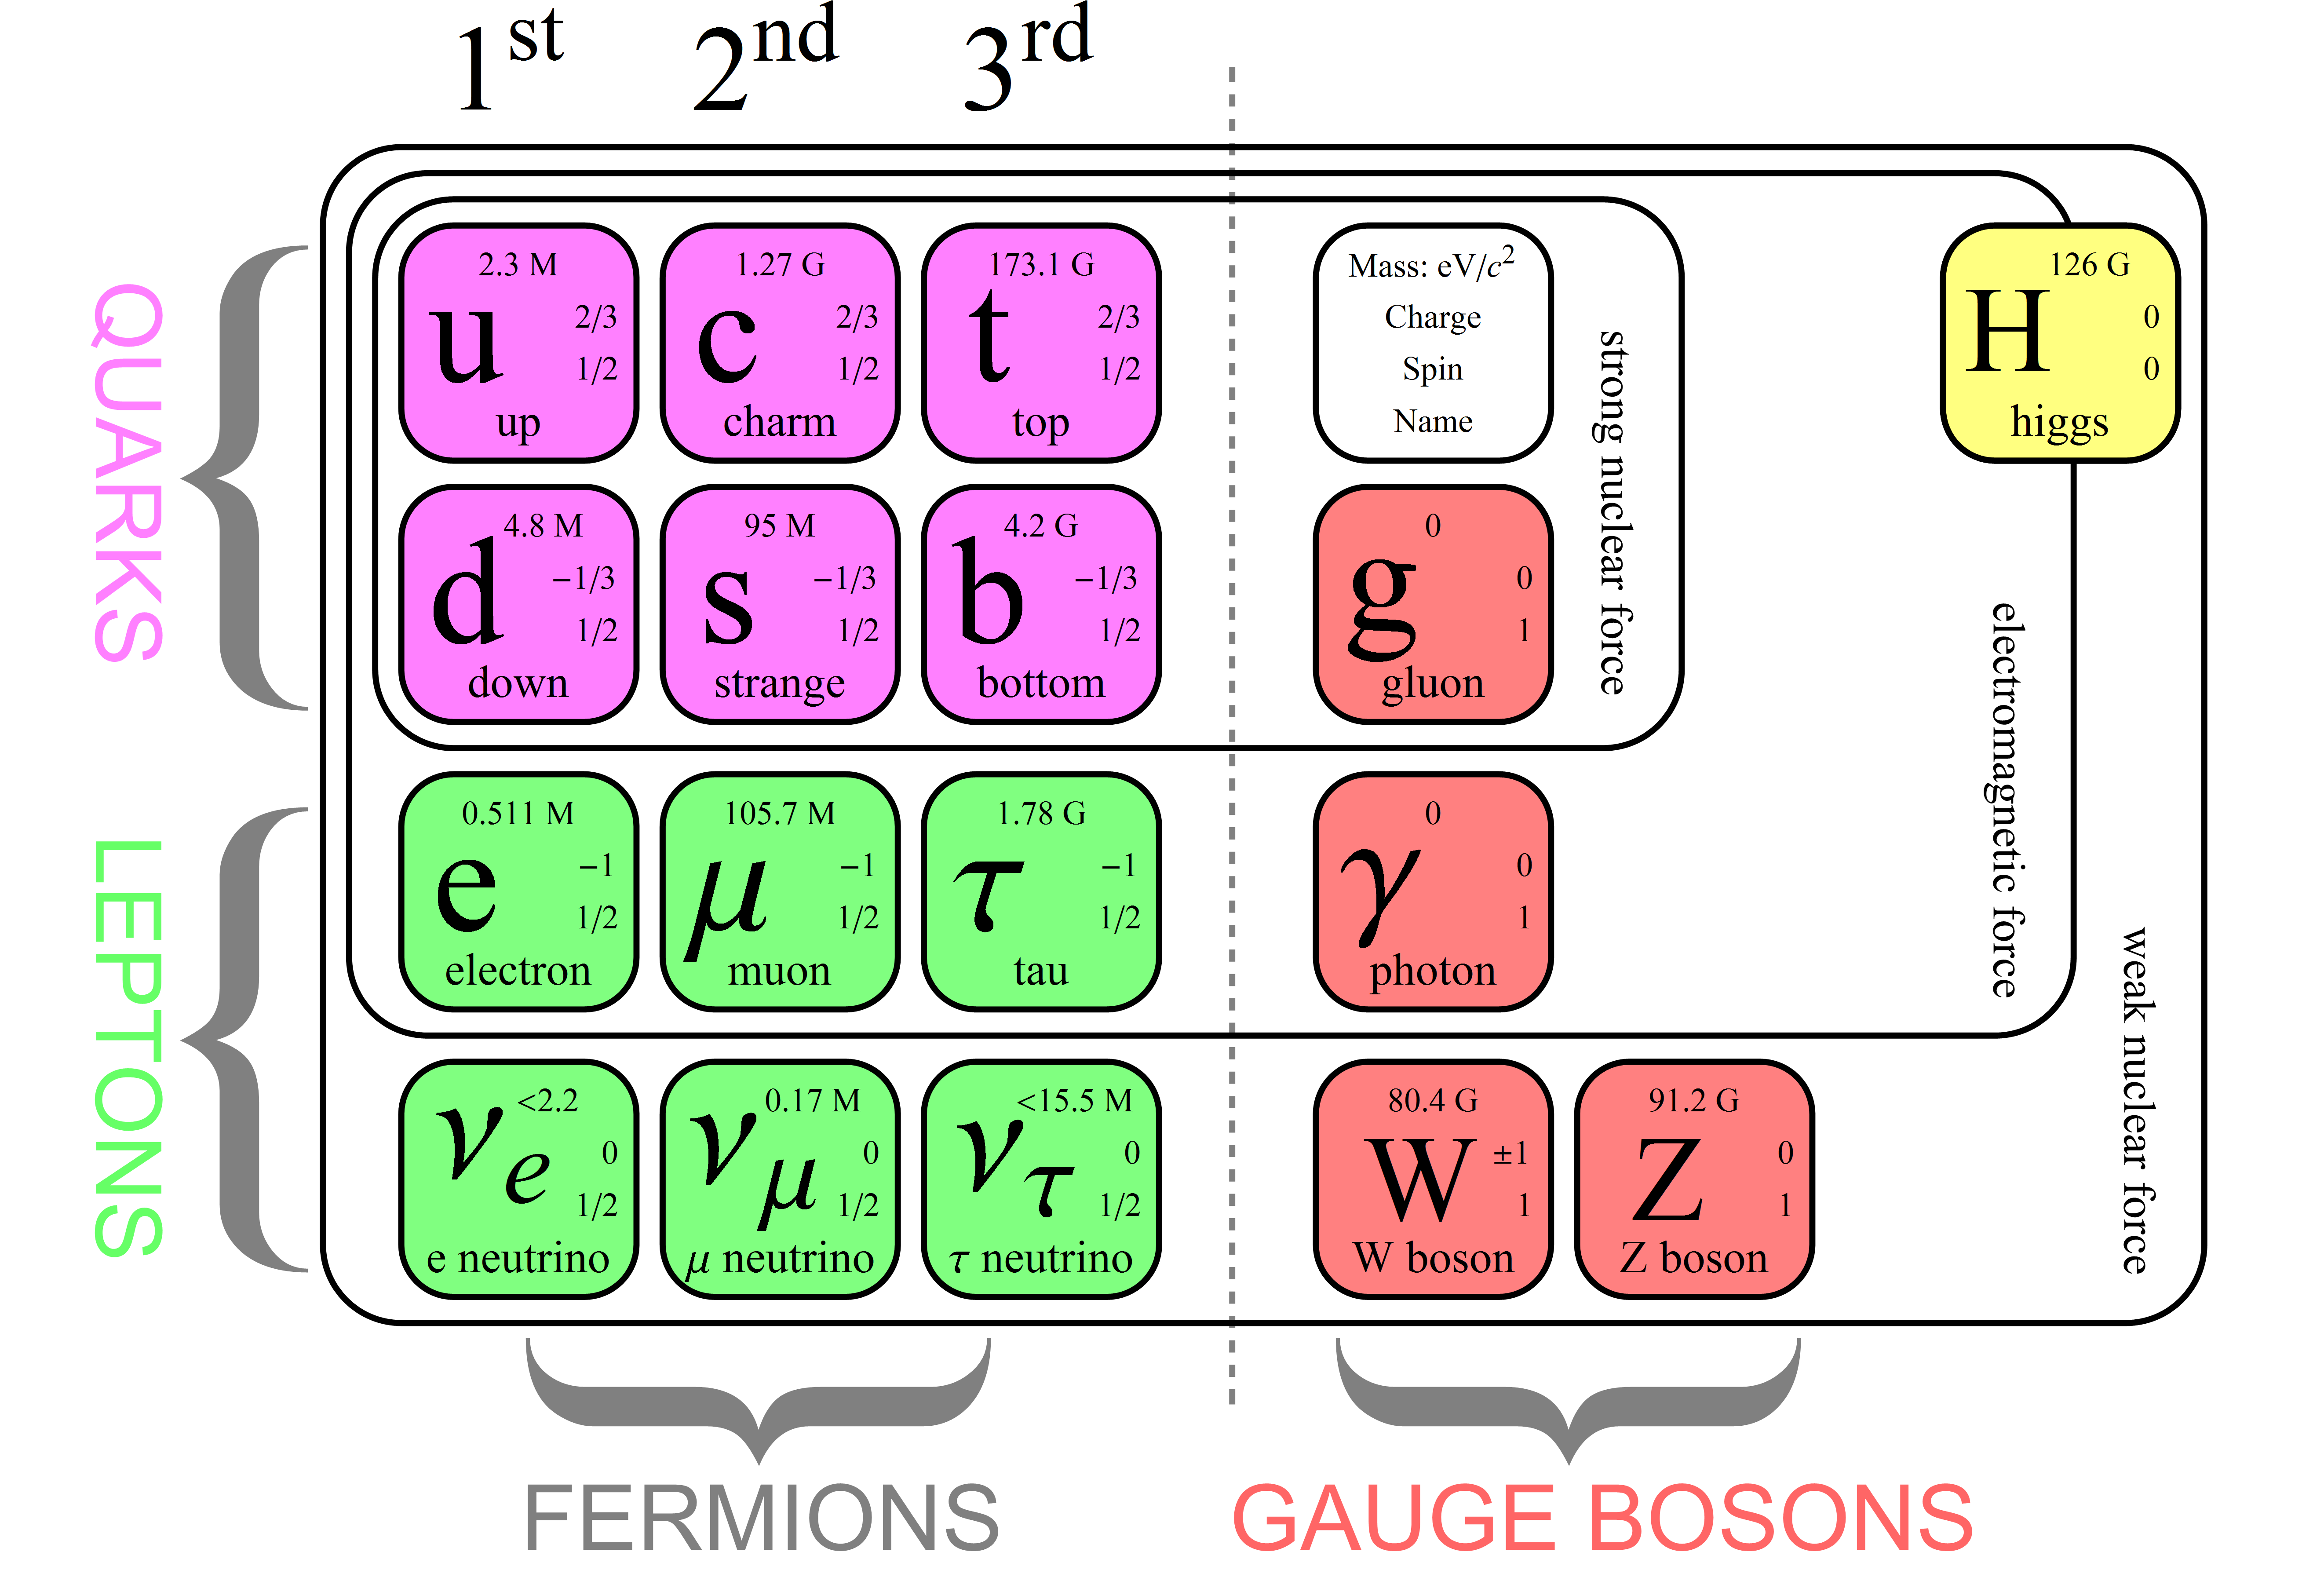
\includegraphics[width = .9\textwidth]{SM_particles.png}
\caption{Figure showing the particles of the Standard Model, and their respective forces. Each column represents a generation of particles.}
\label{fig: SM_particles}
\end{figure}


\section{Feynman Diagrams}
\begin{itemize}
    \item A graphical representation of particle interactions.
    \item Time goes from left to right.
    \item The particles are represented by lines, and the interactions are represented by vertices.
    \item \textbf{Fermions}: 
    \begin{itemize}
        \item Represented by straight lines with arrows
        \item Anti-particles are represented by straight lines with arrows pointing in the opposite direction.
    \end{itemize}
    \item \textbf{Electromagnetic/Weak Interactions}:
    \begin{itemize}
        \item Represented by wavy lines
        \item Virtual photons (often noted by an asterisk) may have mass and may not move at the speed of light
    \end{itemize}
    \item \textbf{Strong Interactions}: Represented by curly lines.
    \item \textbf{Higgs Boson}: Represented by a dashed line.
\end{itemize}

